% !TEX spellcheck = en_US
% !TEX spellcheck = LaTeX
\documentclass[a4paper,10pt,english]{article}
\usepackage{%
	amsfonts,%
	amsmath,%	
	etex,%
	amssymb,%
	amsthm,%
	babel,%
	bbm,%
	%biblatex,%
	caption,%
	centernot,%
	color,%
	enumerate,%
	epsfig,%
	epstopdf,%
	geometry,%
	graphicx,%
	hyperref,%
	latexsym,%
	mathtools,%
	multicol,%
	pgf,%
	pgfplots,%
	pgfplotstable,%
	pgfpages,%
	proof,%
	psfrag,%
	subfigure,%	
	tikz,%
	ulem,%
	url%
}	

\usepackage[mathscr]{eucal}
\usepgflibrary{shapes}
\usetikzlibrary{%
  arrows,%
	backgrounds,%
	chains,%
	decorations.pathmorphing,% /pgf/decoration/random steps | erste Graphik
	decorations.text,%
	matrix,%
  	positioning,% wg. " of "
  	fit,%
	patterns,%
  	petri,%
	plotmarks,%
  	scopes,%
	shadows,%
  	shapes.misc,% wg. rounded rectangle
  	shapes.arrows,%
	shapes.callouts,%
  	shapes%
}

\theoremstyle{plain}
\newtheorem{thm}{Theorem}[section]
\newtheorem{lem}[thm]{Lemma}
\newtheorem{prop}[thm]{Proposition}
\newtheorem{cor}[thm]{Corollary}

\theoremstyle{definition}
\newtheorem{defn}[thm]{Definition}
\newtheorem{conj}[thm]{Conjecture}
\newtheorem{exmp}[thm]{Example}
\newtheorem{assum}[thm]{Assumptions}
\newtheorem{axiom}[thm]{Axiom}

\theoremstyle{remark}
\newtheorem{rem}{Remark}
\newtheorem{note}{Note}

\newcommand{\norm}[1]{\left\lVert#1\right\rVert}
\newcommand{\indep}{\!\perp\!\!\!\perp}
\DeclarePairedDelimiter\abs{\lvert}{\rvert}%
%\DeclarePairedDelimiter\norm{\lVert}{\rVert}%
\newcommand{\tr}{\operatorname{tr}}
\newcommand{\R}{\mathbb{R}}
\newcommand{\Q}{\mathbb{Q}}
\newcommand{\N}{\mathbb{N}}
\newcommand{\E}{\mathbb{E}}
\newcommand{\Z}{\mathbb{Z}}
\newcommand{\B}{\mathscr{B}}
\newcommand{\C}{\mathcal{C}}
\newcommand{\T}{\mathscr{T}}
\newcommand{\F}{\mathcal{F}}
\newcommand{\G}{\mathcal{G}}
%\newcommand{\ba}{\begin{align*}}
%\newcommand{\ea}{\end{align*}}

\makeatletter
\def\th@plain{%
  \thm@notefont{}% same as heading font
  \itshape % body font
}
\def\th@definition{%
  \thm@notefont{}% same as heading font
  \normalfont % body font
}
\makeatother
\date{}
\title{Lecture 02: Poisson Process}
\author{}

\begin{document}
\maketitle

\section{Simple point processes}
\begin{defn} A stochastic process $\{N(t), t\geqslant 0\}$ is a \textbf{point process} if
\begin{enumerate}
  \item $N(0) = 0$, and 
  \item for each $\omega \in \Omega$, the map $t\mapsto N(t)$ is non-decreasing, integer valued, and right continuous.% and at points of discontinuity $(N(t)- N(t^{-}))\leqslant 1,~~\forall \omega \in \Omega$. 
\end{enumerate}
\end{defn} 
\begin{defn} A \textbf{simple point process} is a point process of jump size 1.
\end{defn}

\begin{figure}[hhhh]
\center
	\begin{tikzpicture}
[node distance=1cm, draw=black, thick, >=stealth',
axes/.style=,
codeword/.style={rectangle, draw=black, inner sep=0pt, minimum height=0.8cm, minimum width=0.5cm}]

\begin{scope}[axes]
\draw[->] (0,0) -- (8,0) node[right] {$t$} coordinate (time);
\draw[->] (0,0) -- (0,5) node[above] {$N(t)$} coordinate (number of  events);
\foreach \x/\xtext in {1/S_1, 2/S_2, 5/S_3,7/S_4}
	\draw[xshift=\x cm] (0pt,1pt) -- (0pt,-1pt) node[below,fill=white] {$\xtext$};
\foreach \y/\ytext in {1,...,4}
	\draw[yshift=\y cm] (1pt,0pt) -- (-1pt,0pt) node[left,fill=white] {$\ytext$};
\end{scope}
\draw[] (0,0)--(1,0)--(1,1)--(2,1)--(2,2)--(5,2)--(5,3)--(7,3)--(7,4)--(8,4);
\end{tikzpicture}

	\caption{Sample path of a simple point process.}
	\label{Fig:Poisson}
\end{figure}
\begin{defn} We can define a random variable $S_n$ as the time of $n^{\text{th}}$ discontinuity, written
\begin{xalignat*}{3}
&S_n = \inf\{t \geq 0: N(t) = n\}, n \in \N,&& S_0 = 0.
\end{xalignat*}
The points of discontinuity corresponds to the arrival instants of the point process. 
\end{defn}
\begin{lem} Simple point process $\{N(t), t \geqslant 0\}$ and arrival process $\{S_n: n \in \N\}$ are inverse processes. That is,
\begin{align*}
\{S_n \leqslant t\} = \{N(t) \geqslant n\}.
\end{align*}
\end{lem}
\begin{proof} Let $\omega \in \{S_n \leqslant t\}$, then $N(S_n) = n$. Since $N$ is a non-decreasing process, we have $N(t) \geq N(S_n) = n$. 
%It follows that $\{S_n \leqslant t\} \subseteq \{N(t) \geqslant n\}$.
Conversely, let $\omega \in \{N(t) \geqslant n\}$, then it follows from definition that $S_n \leq t$.
\end{proof}
\begin{cor} The following identity is true.
\begin{align*}
\{S_n \leqslant t, S_{n+1} > t\} = \{N(t) = n\}.
\end{align*}
\end{cor}
\begin{lem}
Let $F_n(x)$ be the distribution function for $S_n$, then 
\begin{align*}
P_n(t) \triangleq \Pr\{N(t) = n\} = F_{n}(t)-F_{n+1}(t).
\end{align*}
\end{lem}
\begin{proof} It suffices to observe that following is a union of disjoint events,
\begin{align*}
\{S_n \leqslant t, S_{n+1} > t\} \cup \{S_{n} \leqslant t, S_{n+1} \leqslant t\} = \{S_n \leqslant t \}.
\end{align*}
\end{proof}
\begin{defn} The inter arrival time between $(n-1)^{th}$ and $n^{th}$ arrival is denoted by $X_n$ and written as
\begin{align*}
X_n = S_n - S_{n-1}.
\end{align*}
\end{defn}
\begin{rem} For a simple point process, we have
\begin{align*}
\Pr\{X_{n} = 0\} &= \Pr\{X_n\leqslant 0\} = 0.
\end{align*}
\end{rem}
\begin{defn} A point process $\{N(t), t\geqslant 0\}$ is called \textbf{stationary increment point process}, if for any collection of $0 < t_{1}<t_{2}, \ldots,<t_{n}$, the joint distribution of $(N(t_{n})-N(t_{n-1}),N(t_{n-1})-N(t_{n-2}),...,N(t_{1}))$ is identical to the joint distribution of $(N(t_{n}+t)-N(t_{n-1}+t),...,N(t_{1}+t)), ~ \forall t \geqslant 0$.
\end{defn}

\begin{defn} A point process $\{N(t), t\geqslant 0\}$ is called \textbf{stationary independent increment process}, if it has stationary increments and the increments are independent random variables.
\end{defn}

\begin{lem} Sequence of inter-arrival times $\{X_n: n \in \N\}$ of a simple stationary independent increment process $\{N(t), t \geqslant 0 \}$ consists of \emph{iid} random variables.
\end{lem}
\begin{proof} It suffices to show that $X_n$ is independent of $S_{n-1}$ to show that all inter-arrival times are independent. 
We see that
%\begin{align*}
%\{S_n \leqslant x, S_{n+1} - S_n > y\} &= \{S_n \leqslant x, N(y+S_n) - N(S_n) = 0\},\\
%&=\{n = N(S_n) \leqslant N(x), N(y+S_n)-N(S_n)\}. 
%\end{align*}
%Further, we observe that
\begin{align*}
\Pr\{S_n \leqslant x, S_{n+1} - S_n > y\} &= \int_{x \leq t}\Pr\{N(y+t) - N(t) = 0|S_n = t\}dF_n(t)\\
&=\int_{x \leq t}\Pr\{N(y+t) - N(t) = 0|N(t) = n \}dF_n(t) = \Pr\{X_n > y\}F_n(x).
\end{align*}
To show that each inter-arrival time is identically distributed, we observe that
\begin{align*}
\Pr\{S_n - S_{n-1} > x\} &= \Pr\{N(x + S_{n-1}) - N(S_{n-1}) > 0\}\\
&= \int_{t > 0}\Pr\{N(x) = 0\}dF_{n-1}(t) = \Pr\{N(x) = 0\}.
\end{align*}
\end{proof}

\section{Poisson process}
\begin{lem} A unique non-negative right continuous function $f: \R \to \R$ satisfying align 
\begin{align*}
 f(t+s) = f(t)f(s), \text{ for all } t,s \in \R
 \end{align*}
 is $f(t) = e^{\theta t}$, where $\theta = \log f(1)$.
\end{lem}
\begin{proof}
Clearly, we have $f(0) = f^2(0)$. Since $f$ is non-negative, it means $f(0) = 1$. By definition of $\theta$ and induction for $m,n \in \Z^+$, we see that 
\begin{xalignat*}{3}
&f(m) = f(1)^m = e^{\theta m},&& e^{\theta} = f(1) = f(1/n)^n.
 \end{xalignat*}
Let $q \in \Q$, then it can be written as $m/n, n \neq 0$ for some $m,n \in \Z^+$. 
Hence, it is clear that for all $q \in \Q^+$, we have $f(q) = e^{\theta q}$.
either unity or zero. Note, that $f$ is a right continuous function and is non-negative. 
%We will show that $g$ is an exponential function. That is, $g(t) = e^{\theta t}$ for some $\theta \geqslant 0$. We will prove this in stages. First, we show this is true for $t \in \mathbb{Z}^+$. Notice that we can obtain via induction
%\begin{eqnarray*}
%	g(2) &=& g(1) g(1) = g^{2}(1), \mathrm{ and }\\
%	g(m) &=& [g(1)]^{m}.
%\end{eqnarray*}
%Since $g(1)$ is non negative, there exists a $\beta$ such that $g(1)=e^{\beta}$ and $g(m)= e^{m \beta}, m \in \mathbb{Z}_{+}$. Next we show that for any $n \in \mathbb{Z}_{+}$,        
%\begin{align*}
%	g(1) =  g\left(\frac{1}{n}+..., +\frac{1}{n}\right) = \left[g\left(\frac{1}{n}\right)\right]^{n}.
%\end{align*}
%Therefore, for same $\beta$ we used for $g(1)$, we have $g\left(\frac{1}{n}\right) = e^{\frac{\beta}{n}}$. Now, we show that $g$ is exponential for any $t \in \mathbb{Q}^+$. To this end, we see that for any $m, n \in \mathbb{Z}_{+}$, we have 
%\begin{align*}
%	g\left(\frac{m}{n}\right) = \left[g\left(\frac{1}{n}\right)\right]^{m}= e^{\frac{m \beta}{n}}.
%\end{align*}
Now, we can show that $f$ is exponential for any real positive $t$ by taking a sequence of rational numbers $\{t_n\}$ decreasing to $t$. From right continuity of $g$, we obtain 
\begin{align*}
	g(t) = \lim_{t_n \downarrow t} g(t_n) =   \lim_{t_n \downarrow t} e^{\beta t_{n}}= e^{\beta t}.
\end{align*}
\end{proof}
\begin{defn} A random variable $X$ with continuous support on $\R_+$, is called \textbf{memoryless} if for all $t,s \in \R_+$, we have
\begin{align*}
  \Pr\{X>s\} &= \Pr\{ X > t+s| X>t\}.% = \frac{ \Pr\{ X>t+s, X>t\}}{\Pr\{X>t\}}.
\end{align*}
\end{defn}
\begin{prop} The unique memoryless distribution function with continuous support on $\R_+$ is the exponential distribution.
\end{prop}
\begin{proof}
Let $X$ be a random variable with a distribution function $F: \R_+ \to [0,1]$ with the memoryless property. Let $g(t) \triangleq 1 - F(t)$. It follows from the memoryless property of $F$, that
\begin{align*}
 g(t+s) = g(t)g(s).
 %\Pr\{X>s\} &= \Pr\{ X > t+s| X>t\} \\&= \frac{ \Pr\{ X>t+s, X>t\}}{\Pr\{X>t\}}.
\end{align*}
%Since $\{X > t + s\} =\{ X>t+s, X>t\}$, we have $g(t+s) = g(t)g(s)$ and hence $g(0) = g^2(0)$. Therefore, $g(0)$ is either unity or zero. Note, that $g$ is a right continuous function and is non-negative. 
%
%We will show that $g$ is an exponential function. That is, $g(t) = e^{\theta t}$ for some $\theta \geqslant 0$. We will prove this in stages. First, we show this is true for $t \in \mathbb{Z}^+$. Notice that we can obtain via induction
%\begin{eqnarray*}
%	g(2) &=& g(1) g(1) = g^{2}(1), \mathrm{ and }\\
%	g(m) &=& [g(1)]^{m}.
%\end{eqnarray*}
%Since $g(1)$ is non negative, there exists a $\beta$ such that $g(1)=e^{\beta}$ and $g(m)= e^{m \beta}, m \in \mathbb{Z}_{+}$. Next we show that for any $n \in \mathbb{Z}_{+}$,        
%\begin{align*}
%	g(1) =  g\left(\frac{1}{n}+..., +\frac{1}{n}\right) = \left[g\left(\frac{1}{n}\right)\right]^{n}.
%\end{align*}
%Therefore, for same $\beta$ we used for $g(1)$, we have $g\left(\frac{1}{n}\right) = e^{\frac{\beta}{n}}$. Now, we show that $g$ is exponential for any $t \in \mathbb{Q}^+$. To this end, we see that for any $m, n \in \mathbb{Z}_{+}$, we have 
%\begin{align*}
%	g\left(\frac{m}{n}\right) = \left[g\left(\frac{1}{n}\right)\right]^{m}= e^{\frac{m \beta}{n}}.
%\end{align*}
%Now, we can show that $g$ is exponential for any real positive $t$ by taking a sequence of rational numbers $\{t_n\}$ decreasing to t. From right continuity of $g$, we obtain 
%\begin{align*}
%	g(t) \stackrel{(a)}{=} \lim_{n\rightarrow \infty} g(t_n) =   \lim_{n\rightarrow \infty} e^{\beta t_{n}}= e^{\beta t}.
%\end{align*}
Since $g(x) = \Pr\{X > x\}$  is non-increasing  with $x \in \R_+$, we have $g(x) = e^{\theta x}$, where $\theta < 0$.
\end{proof}

\begin{defn} A simple point process $\{N(t),~ t\geqslant 0\} $ is called a \textbf{Poisson process} with a finite positive rate $\lambda$, if inter-arrival times $\{X_{n}: n \in \N\}$ are \emph{iid} random variables with an exponential distribution of rate $\lambda$. That is, it has a distribution function $F$, such that 
 \begin{align*}
 F(x) = \Pr\{X_{1}\leqslant x\} = 
	\begin{cases}
		1-e^{-\lambda x}, & x\geqslant 0   \\
		0,  & \text{ else}.
	\end{cases}
\end{align*}
\end{defn}

\begin{thm} A simple stationary independent increment process is a Poisson process with parameter $\lambda$ when
\begin{xalignat*}{3}
&\lim_{t \to 0}\frac{\Pr\{N(t) = 1\}}{t} = \lambda,&&\lim_{t \to 0}\frac{\Pr\{N(t) \geq 2\}}{t} = 0.
\end{xalignat*}
\end{thm}
\begin{proof}
It suffices to show that first inter-arrival times $X_1$ is exponentially distributed with parameter $\lambda$. Notice that
\begin{align*}
P_0(t+s) = \Pr\{N(t+s) - N(t) = 0, N(t) = 0\} = P_0(t)P_0(s).
\end{align*}
Using the conditions in the theorem, the result follows.
\end{proof}
\subsection{Distribution functions}
\begin{lem} Moment generating function of arrival times $S_n$ is 
 \begin{align*}
  \mathbb{E} [ e^{\theta S_n} ] = 
		\begin{cases}
		\frac{\lambda^n}{(\lambda-\theta)^n}, & \theta < \lambda \\
		\infty, & \theta \geqslant \lambda.
		\end{cases} 
 \end{align*} 
 Distribution function of $S_n$ is given by 
 \begin{align*}.
 \end{align*}
\end{lem}
\begin{proof} 
Since $S_n = \sum_{k=1}^nX_k$, where $X_k$ are \emph{iid}, the moment generating function $\mathbb{E} [ e^{\theta S_{n}} ]$ of $S_n$ is 
 \begin{align*}
  \mathbb{E} [ e^{\theta S_{n}} ] = \left(\mathbb{E}[e^{\theta X_{1}}]\right)^{n}. 
 \end{align*} 
Since each $X_k$ is \emph{iid} exponential with rate $\lambda$, it is easy to see that moment generating function of inter-arrival time $X_1$ is 
 \begin{align*}
  \mathbb{E} [ e^{\theta X_1} ] = 
		\begin{cases}
		\frac{\lambda^n}{(\lambda-\theta)^n}, & \theta < \lambda \\
		\infty, & \theta \geqslant \lambda.
		\end{cases} 
 \end{align*} 
\end{proof}

\begin{thm} Density function of $S_n$ is Gamma distributed with parameters $n$ and $\lambda$. That is,
\begin{align*}
f_{n}(s) =\frac{\lambda (\lambda s)^{n-1}} {(n-1)!} e^{-\lambda s}.
\end{align*}
\end{thm}
\begin{proof} Notice that $X_i$'s are \emph{iid} and $S_1 = X_1$. In addition, we know that $S_n = X_n + S_{n-1}$. Since, $X_n$ is independent of $S_{n-1}$, we know that distribution of $S_n$ would be convolution of distribution of $S_{n-1}$ and $X_1$. Since $X_n$ and $S_1$ have identical distribution, we have $f_{n}=f_{n-1}*f_{1}$. The result follows from straightforward induction.
\end{proof}

%Process $N(t)$ is of real interest, and we can compute the distribution of $N(t)$ for each $t$ from the distribution of $S_n$ in the following.
%\begin{figure}[hhhh]
%\center
	%\begin{tikzpicture}
[node distance=1cm, draw=black, thick, >=stealth',
axes/.style=,
codeword/.style={rectangle, draw=black, inner sep=0pt, minimum height=0.8cm, minimum width=0.5cm}]

\begin{scope}[axes]
\draw[->] (0,0) -- (8,0) node[right] {$t$} coordinate (time);
\draw[->] (0,0) -- (0,5) node[above] {$N(t)$} coordinate (number of  events);
\foreach \x/\xtext in {1/S_1, 2/S_2, 5/S_3,7/S_4}
	\draw[xshift=\x cm] (0pt,1pt) -- (0pt,-1pt) node[below,fill=white] {$\xtext$};
\foreach \y/\ytext in {1,...,4}
	\draw[yshift=\y cm] (1pt,0pt) -- (-1pt,0pt) node[left,fill=white] {$\ytext$};
\end{scope}
\draw[] (0,0)--(1,0)--(1,1)--(2,1)--(2,2)--(5,2)--(5,3)--(7,3)--(7,4)--(8,4);
\end{tikzpicture}

 %% \caption{}\label{}
%\end{figure}
\begin{thm} For each $t >0$, the distribution of Poisson process $N(t)$ with parameter $\lambda$ is given by
	\begin{align*}
	\Pr\{N(t)=n)\}= e^{-\lambda t}\frac{(\lambda t)^{n}}{n!}.
	\end{align*}
Further, $E[N(t)] = \lambda t$, explaining the rate parameter $\lambda$ for Poisson process.
\end{thm}
\begin{proof}
Result follows from density of $S_n$ and recognizing that 
\begin{align*}
P_n(t) = F_n(t) - F_{n+1}(t).
\end{align*}
%\begin{eqnarray*}
%   \Pr\{N(t) =n\}&=&  \Pr\{S_{n}\leqslant t, S_{n+1} >t)\\
%   &=&  \int^{t}_{0} \Pr\left\{ {S_{n+1}>t}|{S_{n}=s}\right\}f_{n}(s)  ds\\
%   &\stackrel{(a)}{=}& \int^{t}_{0} \Pr\{X_{n+1}>t-s\} f_{n}(s) ds\\
%   &=&  \int^{t}_{0}e^{-\lambda(t- s)} \frac{\lambda^{n}s^{n-1}}{(n-1)!}e^{-\lambda s}  ds\\
%   &=&\frac{e^{-\lambda t} (\lambda t)^{n}}{n !}.
%\end{eqnarray*}
% where (a) follows from the memoryless property of exponential distribution. %($\Pr\{X_{n+1}>s+t|X_{k+1}>t)=\Pr\{X_{k+1}>s)$).\\
\end{proof}

\begin{cor} Distribution of arrival times $S_n$ is 
\begin{align*}
	F_n(t)= \sum_{j \geq n}e^{-\lambda t}\frac{(\lambda t)^{j}}{j!}.
\end{align*}
Further, $\sum_{n \in \N_0}F_n(x) = 1 + \lambda t$.
\end{cor}
\begin{proof}
Result follows from distribution of $P_n(t)$ and recognizing that $F_n(t) =  \sum_{j \geq n}P_j(t)$.
Further, we notice that
\begin{align*}
\sum_{n \in \N_0}F_n(t) &=  \sum_{n \in \N_0}\sum_{j \geq n}P_j(t) = \sum_{i \in \N_0}\sum_{n = 0}^{j}P_j(t) = \sum_{i \in \N_0}(j+1)P_j(t)\\
&= 1 + E[N(t)] = 1 + \lambda t.
\end{align*}
\end{proof}


\begin{rem} A Poisson process is not a stationary process. That is, the finite dimensional distributions are not shift invariant. 
\end{rem}
%In the following section, we show that the Poisson process is a \textit{stationary,  independent increment} process. To this end, we will use an important property of exponential distribution- namely memoryless property. Memoryless property of exponential distribution will facilitate the computation of fdd of the Poisson process via one dimensional marginal distribution. 
\begin{lem} For any finite time $t > 0$, a Poisson process is finite almost surely.
\end{lem}
\begin{proof} By strong law of large numbers, we have 
\begin{align*}
\lim_{n \to \infty} \frac{S_{n}}{n} = E[X_{1}] = \frac{1}{\lambda}\quad\mathrm{a.s.} 
\end{align*}
%Therefore, we have $S_n \rightarrow \infty$, a.s. This implies $\Pr\{N(t) < \infty\} =1$. To see this, 
Fix $t > 0$ and let $M = \{\omega \in \Omega: N(t)(\omega) = \infty \}$ be a subset of the sample space. Let $\omega \in M$, then $S_{n}(\omega)\leqslant t$ for all $n \in \N$. This implies $\lim\sup_n\frac{S_{n}}{n} = 0$  and $\omega \not\in \{\lim_n \frac{S_{n}}{n} = \frac{1}{\lambda} \}.$ Hence, the probability measure for set $M$ is zero. 
\end{proof}

\begin{figure}[hhhh]
\center
	\begin{tikzpicture}
[node distance=1cm, draw=black, thick, >=stealth',
axes/.style=,
codeword/.style={rectangle, draw=black, inner sep=0pt, minimum height=0.8cm, minimum width=0.5cm}]

\begin{scope}[axes]
\draw[->] (0,0) -- (9,0) node[right] {$t$} coordinate (time);
\draw[->] (0,0) -- (0,8) node[above] {$N(t)$} coordinate (number of  events);
\foreach \x/\xtext in {0.5/S_{n-3}, 1.5/S_{n-2}, 2.2/S_{n-1},3.2/S_{n}, 4/t_1, 5.1/S_{n+1}, 6/S_{n+2}, 7/t}
	\draw[xshift=\x cm] (0pt,1pt) -- (0pt,-1pt) node[below,fill=white] {$\xtext$};
\foreach \y/\ytext in {1/n-3,2/n-2, 3/n-1, 4/n,5/n+1,6/n+2,7/n+3}
	\draw[yshift=\y cm] (1pt,0pt) -- (-1pt,0pt) node[left,fill=white] {$\ytext$};
\end{scope}
\draw[] (0,0)--(.5,0)--(.5,1)--(1.5,1)--(1.5,2)--(2.2,2)--(2.2,3)--(3.2,3)--(3.2,4)--(5.1,4)--(5.1,5)--(6,5)--(6,6)--(7.5,6)--(7.5,7)--(9,7);
\draw[<->] (4,0) -- node[midway,left]{$N({t_1})$}(4,4);
\draw[<->] (7,0) -- node[midway,left]{$N(t)$}(7,6);
\draw[<->] (3.2,4.1)--node[near start, above]{$X'_{n+1}$}(4,4.1);
\draw[<->] (4,4.1) --node[midway,above]{$X''_{n+1}$}(5.1,4.1);
\end{tikzpicture}

  	\caption{Stationary independent increment property of Poisson process.}
	\label{Fig:IndependentIncrements}
\end{figure}
\begin{prop} A Poisson process $\{N(t), t\geqslant 0\}$ is simple point process with stationary independent increments.
\end{prop}
\begin{proof}
It is clear that Poisson process is a simple point process. 
To show that $N(t)$ has stationary independent increment property, it suffices to show that $N_t-N(t_{1}) \perp N(t_1)$ and $N(t) - N(t_1) \sim N(t-t_1)$. 
This follows from the fact that we can use induction to show stationary independent increment property for for any finite disjoint time-intervals.

Let arrival time-instants $\{S_n: n \in \N_0\}$ and inter-arrival times $\{X_n: n \in \N\}$ be defined as before. 
Given any time $t_1$, we can define the following variables
\begin{xalignat*}{3}
&X'_{N(t_1)+1} = t_1 - S_{N(t_1)},&&X''_{N(t_1)+1} = S_{N(t_1)+1} - t_1.
\end{xalignat*}
It is clear that $t_1$ partitions $X_{N(t_1)+1}$ in two parts such that $X_{N(t_1)+1} = X^{'}_{N(t_1)}+1 + X^{''}_{N(t_1)+1}$ as seen in Figure~\ref{Fig:IndependentIncrements} for the case when $N(t_1) = n$. 
We look at joint distribution of $X'_{N(t_1)+1}, X''_{N(t_1)+1}$ and notice that
\begin{align*}
\{X'_{N(t_1)+1}  > x, X''_{N(t_1)+1} > y\} %&= \bigcup_{n \in \N_0}\{X' \leq x, X'' > y, N(t_1) = n\},\\
&= \bigcup_{n \in \N_0}\{ S_n <  t_1 -x , S_{n+1} > t _1 + y, N(t_1) = n\}\\
&= \bigcup_{n \in \N_0}\{ S_n <  t_1 -x , S_{n+1} > t _1 + y\}.
\end{align*}
From the fact that inter-arrival times are \emph{iid} exponentially distributed with rate $\lambda$, we conclude that
\begin{align*}
\Pr\{X'_{N(t_1)} > x, X''_{N(t_1)+1} > y\} &= \sum_{n \in \N_0}\int_{u=0}^{t_1-x}\Pr\{X_{n+1} > t _1 + y + u \}dF_n(u),\\
&= \int_{u=0}^{t_1-x}(1 - F_1(t_1+y+u))\sum_{n \in \N_0}dF_n(u) = \int_{u=0}^{t_1-x}e^{-\lambda(t_1+y+u)}\lambda du,\\
&= (1-F_1(y))(F_1(t_1) - F_1(2t_1-x)).
\end{align*}
Therefore,  $X_{N(t_1)+1}^{''}$ is independent of $X_{N(t_1)+1}^{'}$ and has same distribution as $X_{n+1}$. 
The memoryless property of exponential distribution is crucially used. 
Further, we see that independent increment holds only if inter-arrival time is exponential. 
Therefore, 
\begin{align*}
\{ N(t_1) = n \} &\iff  \{ S_n = t_1 + X'_{n+1} \}, \\
\{ N(t) - N(t_1) \geqslant m \} &\iff \{ X''_{n+1} + \sum_{i=n+2}^{n+m} X_i \leqslant t - t_1 \}.
\end{align*}
Since, $\{X_i: i \geqslant n+2\}\cup\{X_{n+1}^{''}\}$ are independent of $\{X_i: i \leqslant n\}\cup{X_{n+1}^{'}}$, we have $N(t)-N(t_{1}) \perp N(t_1)$. Further, since $X_{n+1}^{''}$ has same distribution as $X_{n+1}$, we get $N(t) - N(t_1) \sim N(t-t_1)$. By induction we can extend this result to $(N(t_{n})-N(t_{n-1}),...,N(t_{1}))$. 
\end{proof}

\begin{prop} Let $t_0 = 0$, and $\{t_i: 1 \leq i \leq k\}$ be an increasing sequence. A stationary independent increment point process $\{N(t),~t\geqslant 0\}$, such that $N(0) = 0$ is Poisson process iff 
%\begin{figure}[h!]
%\center
  %% Requires \usepackage{graphicx}
  %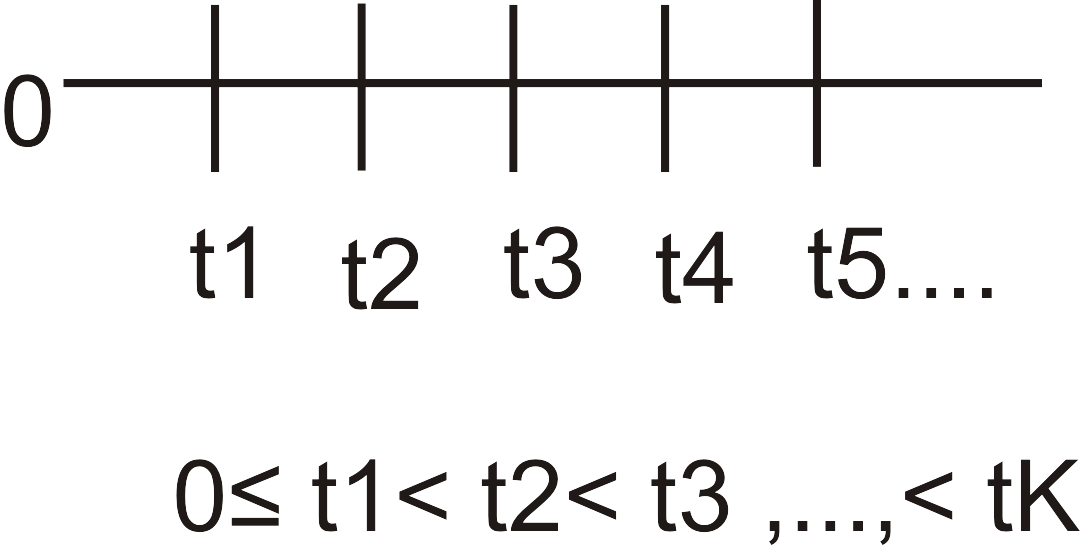
\includegraphics[width=2.8in, height=0.9in]{Figures/SPQT.png}\\
 %% \caption{}\label{}
%\end{figure}
\begin{align*}
  \Pr\{\bigcap_{i=1}^k \{N(t_i)-N(t_{i-1})= n_{i}\}\} = \prod_{i=1}^{k}\frac{(\lambda(t_{i}-t_{i-1}))^{n_{i}}}{n_{i}!} e^{-\lambda (t_{i}-t_{i-1})}.
\end{align*}
\end{prop}
\end{document}